% Due to the increasing amount of students at the Technical University of Munich, the fire evacuation plan for the MI building needs to be reconsidered. An important information is the distribution of people within the MI building p(x). In a hypothetical scenario, the fire department decided to track 100 random students and employees during the busiest hour on different days. The idea is to use this data for learning p(x). As a first experiment, the fire department wants to estimate the number of people that is critical for the building. To simplify the task, it defined a sensitive area in front of the main entrance|marked by the orange rectangle (130/70 & 150/50)| where the number of people should not exceed 100. You will get points for this task if you document the experiments.

% 1. Download the FireEvac dataset (training: 3000 x-y-positions; testing: 600 x-y-positions) and make a scatter plot to visualise it.

Task 4 is centered around reconsidering the current fire evacuation plan for the MI building at the Technical University of Munich. Initially, we download the FireEvac dataset, provided as Numpy \cite{harris2020array} files. Train and test data are loaded into Jupyter Notebook \cite{Kluyver2016jupyter} with the command \texttt{np.load}. Once the data was split into x and y values, we can visualise it with a scatter plot, as can be seen in figure \ref{fig:scatter1}. The left subfigure displays the training data which holds 3000 x-y-positions and thus has more dense positions than the test data on the right with only 600 x-y-positions. Both plots show the possible positions of pedestrians and outline the form of the MI building. 

\begin{figure}[H]
    \centering
    \begin{subfigure}[b]{0.45\textwidth}
        \centering
        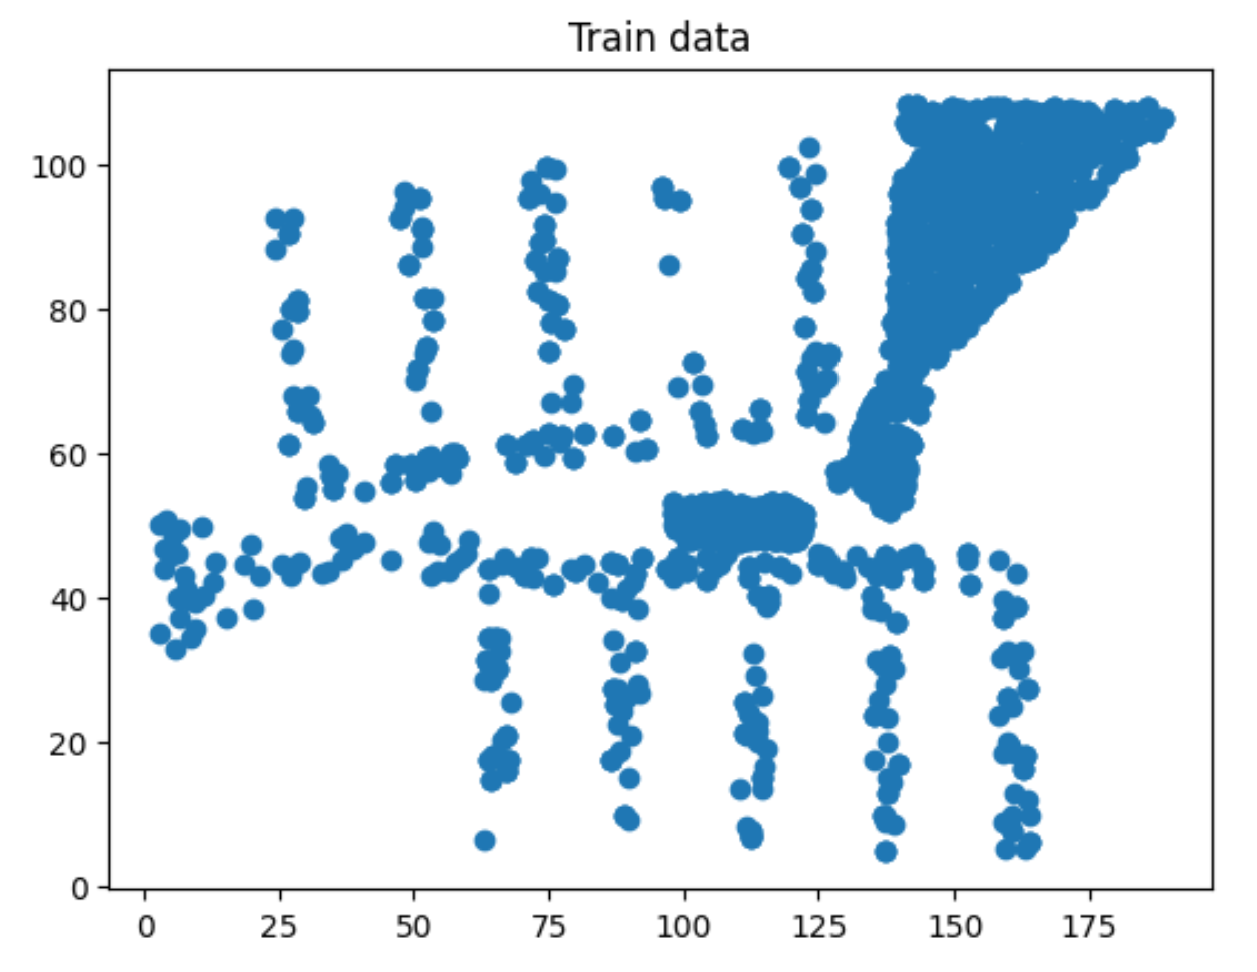
\includegraphics[width=\textwidth]{images/3-scatterTrain.png}
    \end{subfigure}
    \begin{subfigure}[b]{0.45\textwidth}
        \centering
        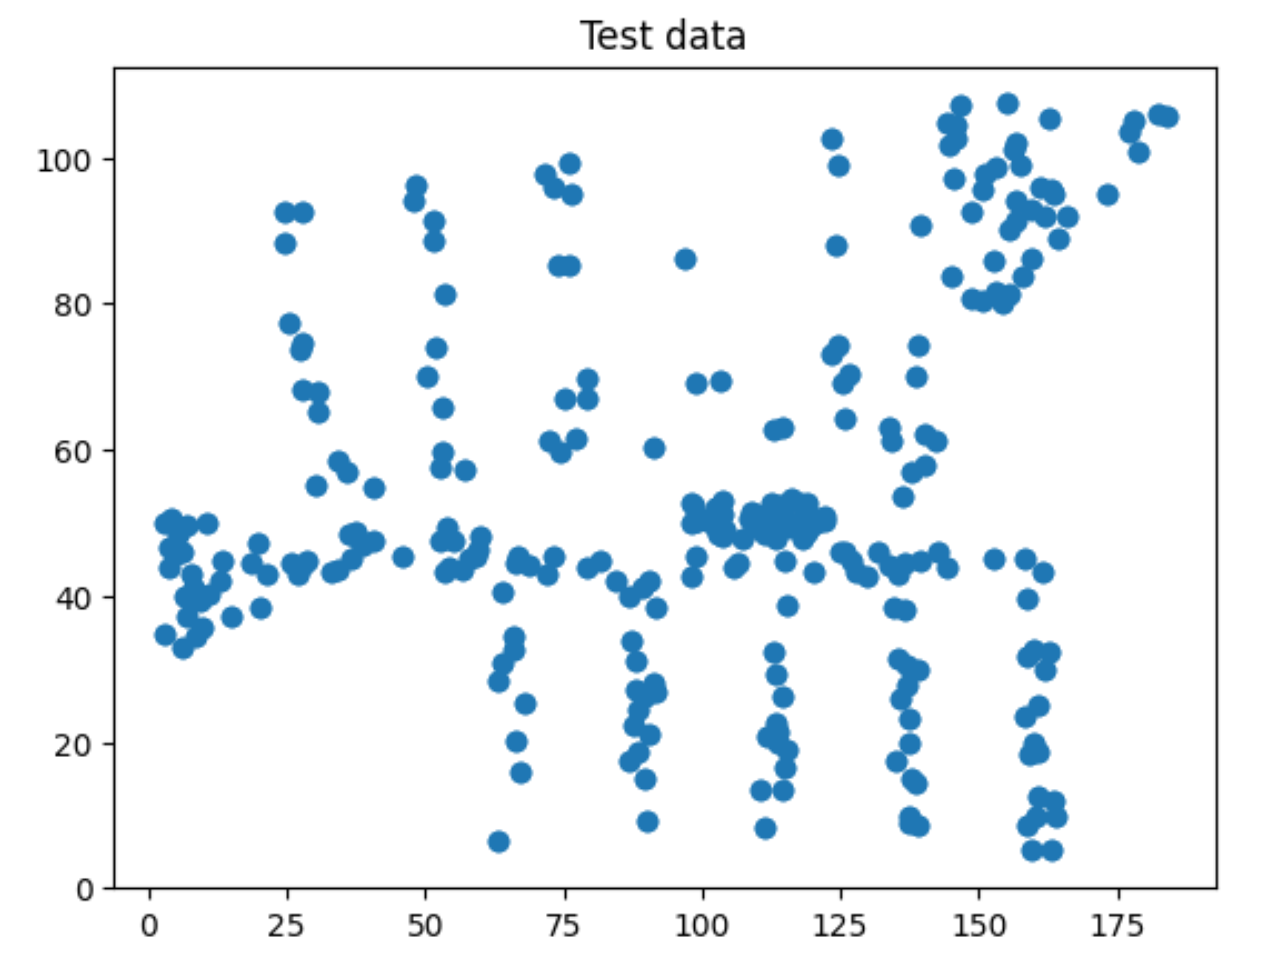
\includegraphics[width=\textwidth]{images/3-scatterTest.png}
    \end{subfigure}
    \caption{Scatter Plot of training and test data before scaling}
    \label{fig:scatter1}
\end{figure}

% Train a VAE on the FireEvac data to learn p(x) (reuse your VAE implementation).
As we want to learn the distribution of people within the MI building $p(x)$, we train a VAE on the FireEvac data. The implementation remains the same as in Task 3 with the exception of a few parameters so that the model can fit the new data better. 

% Make a scatter plot of the reconstructed test set.

\begin{figure}[H]
    \centering
    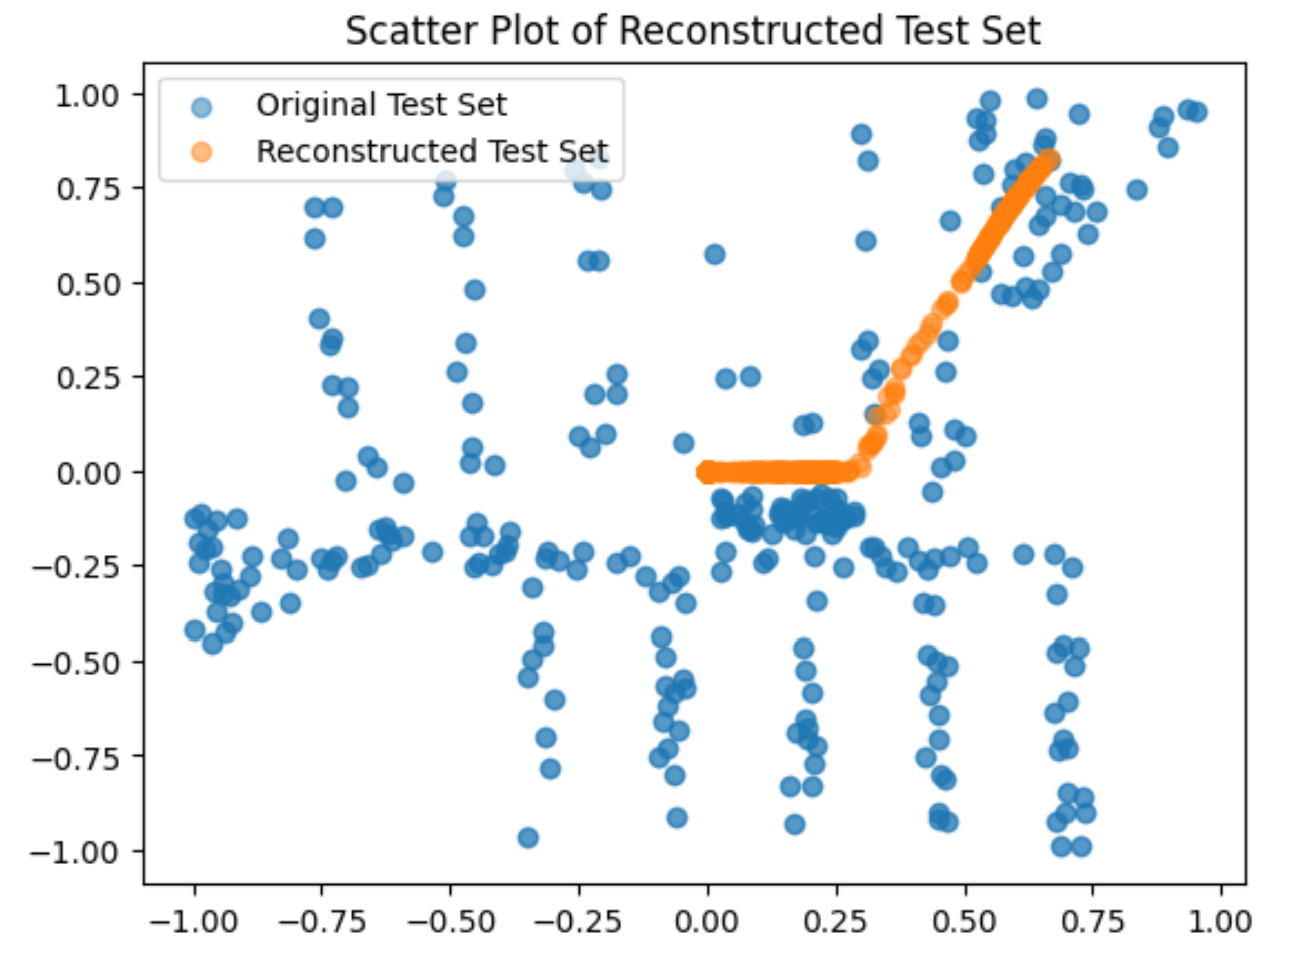
\includegraphics[width=0.7\textwidth]{images/3-scatterReconstructed.png}
    \caption{Comparison of the original and reconstructed test set}
    \label{fig:scatterReconstructed}
\end{figure}

While the reconstructed test set in figure \ref{fig:scatterReconstructed} does not represent the complete original test set well, it does visualise the entrance of the MI building. 
Similarly, figure \ref{fig:scatterGenerated} also depicts the entrance only. Since there is no comparison here, the image is scaled to start at 0.0. 

% Make a scatter plot of 1000 generated samples.
\begin{figure}[H]
    \centering
    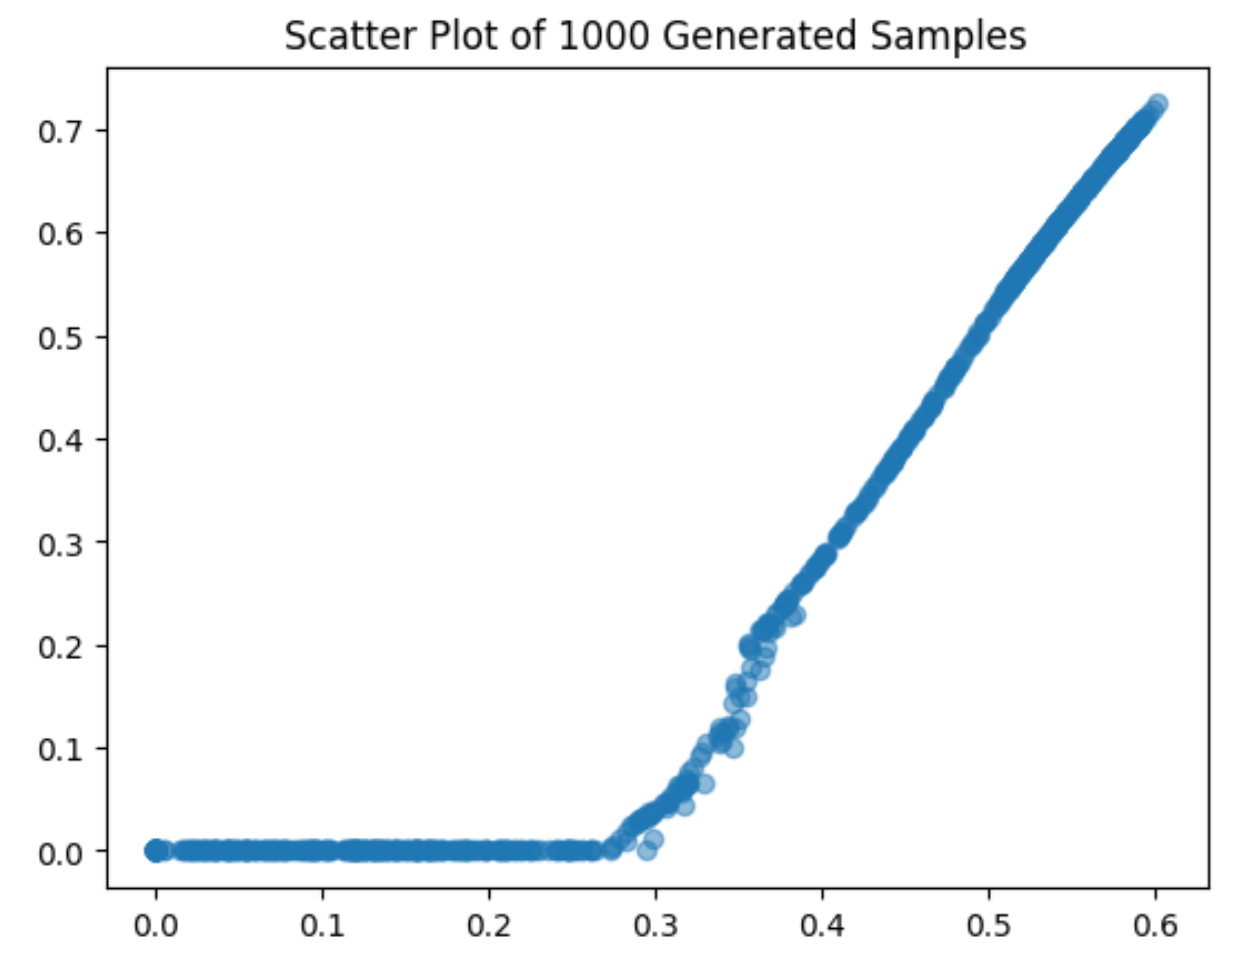
\includegraphics[width=0.7\textwidth]{images/3-scatterGenerated.png}
    \caption{Generated pedestrians in the MI building}
    \label{fig:scatterGenerated}
\end{figure}

% Generate data to estimate the critical number of people for the MI building.
The rectangle in figure \ref{fig:scatterGenRect} defines a sensitive area in front of the main entrance where the number of people should not exceed 100. Since the generated samples follow a straight line instead of scatter in a defined area, only a few pedestrians enter the rectangle on its left top. After increasing the number of generated samples to 5000, the critical number of 100 is surpassed.  

\begin{figure}[H]
    \centering
    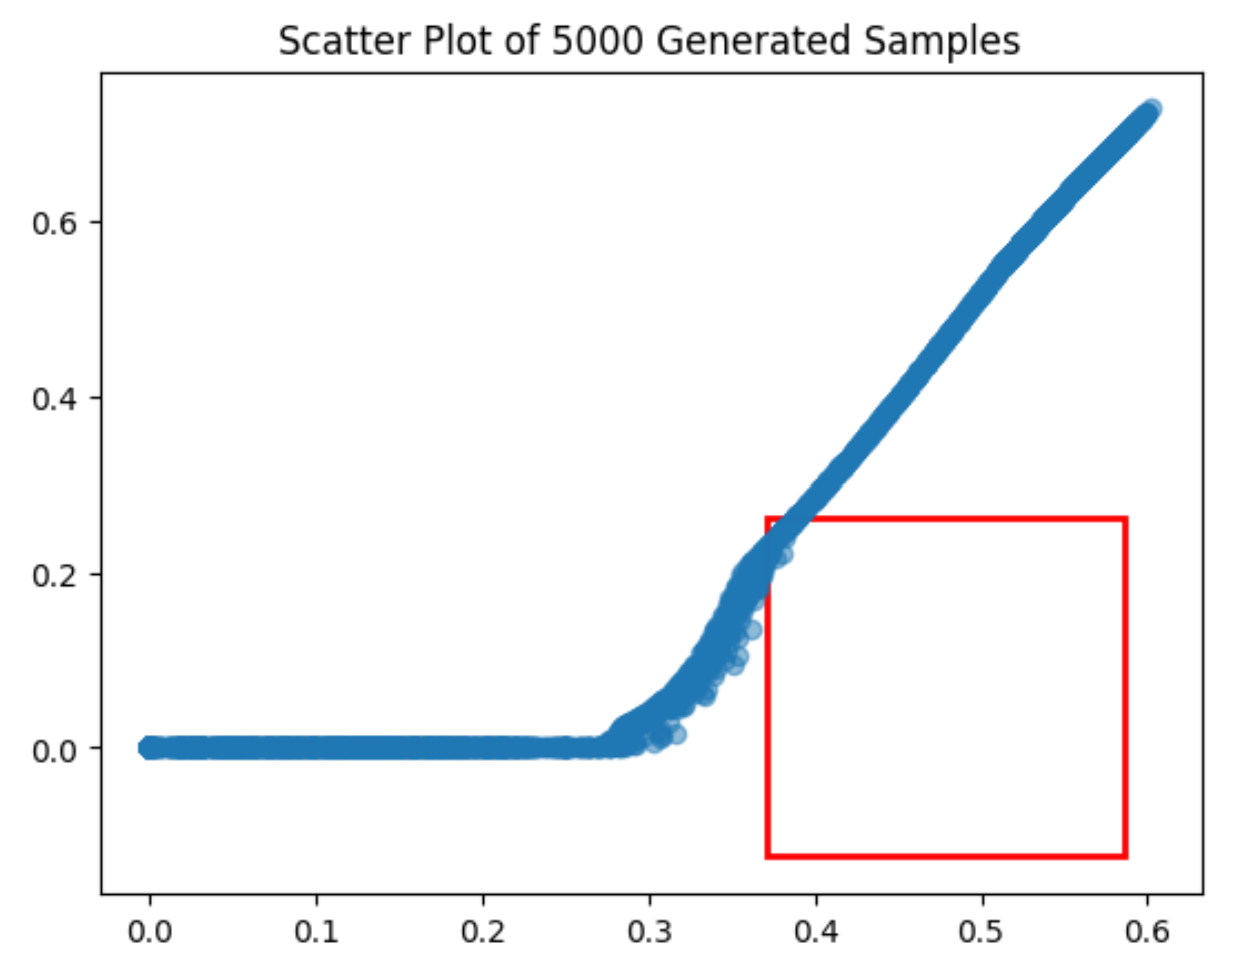
\includegraphics[width=0.7\textwidth]{images/3-scatterGenRect.png}
    \caption{Generated pedestrians (blue) and the sensitive area (red)}
    \label{fig:scatterGenRect}
\end{figure}
% How many samples (people) are needed to exceed the critical number at the main entrance?

% ???
% time estimate
% accuracy
% what we learned

% Verbose discussion of the results in the report?
% Code: modular, concise, well documented?

% Bonus: Use p(x) to sample the positions of 100 people...
% Bonus:...then simulate their trajectories with Vadere as they move toward the target.